\documentclass{article}
\usepackage{xeCJK}
\usepackage{graphicx}
\graphicspath{{figures/}}
\usepackage{float}
\usepackage{amsmath}
\begin{document}
	\section{排队论基础}
	 \textbf{资源的有限性} 和\textbf{ 需求的随机性} 是 排队现象存在的基础;\\
	  由于 顾客到达 和 服务完毕的时间 都是 不确
	 定 的,绝大多数排队系统工作于 随机状态。
	 \section{排队论的概念}
	 \subsection{基本概念}
	 \subsubsection{三个参数}
	 \begin{itemize}
	 	\item  服务员数目m
	 	\item 顾客到达率 $\lambda$ ,相邻两顾客到达的时间间隔$t$,其$\textnormal{统计平均值}\overline{t}=\frac{1}{\lambda}$
	 	\item 服务员服务速率$\mu$ ,顾客服务时间$\tau$,其统计平均值为$\overline{\tau}=\frac{1}{\mu}$\begin{itemize}
	 		\item m = 1,$\mu$为服务速率
	 		\item m >1 ,$m\mu$为服务速率
	 	\end{itemize}
	 \end{itemize}
 	\subsubsection{一般性质}
 	\begin{itemize}
 		\item 平稳性,在时间间隔t内,到达 到达k 个顾客的概率只与t的长 的长
 		度 有关,而与这间隔的起始时刻无关。
 		\item 无后效性,顾客到达时刻互相独立,即顾客各自独立地
 		随机到达。
 		\item 疏稀性,在$\delta t$ 内只有一个顾客到达或没有顾客到达。
 	\end{itemize}
 	满足上三个条件的随机流成为\textbf{简单流},简单流的到达间隔是负指数分布,在一段时间内到达的顾客数服从泊松分布。
	\begin{figure}
		\centering
		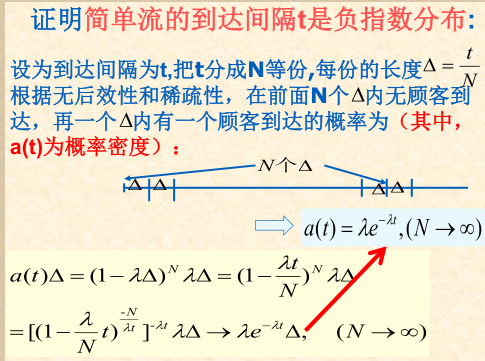
\includegraphics[width=0.7\linewidth]{../通信网路理论基础/chapter2/figures/prove_1}
		\caption{}
		\label{fig:prove1}
	\end{figure}
	
\end{document}